
\begin{SCfigure*}
	\centering
	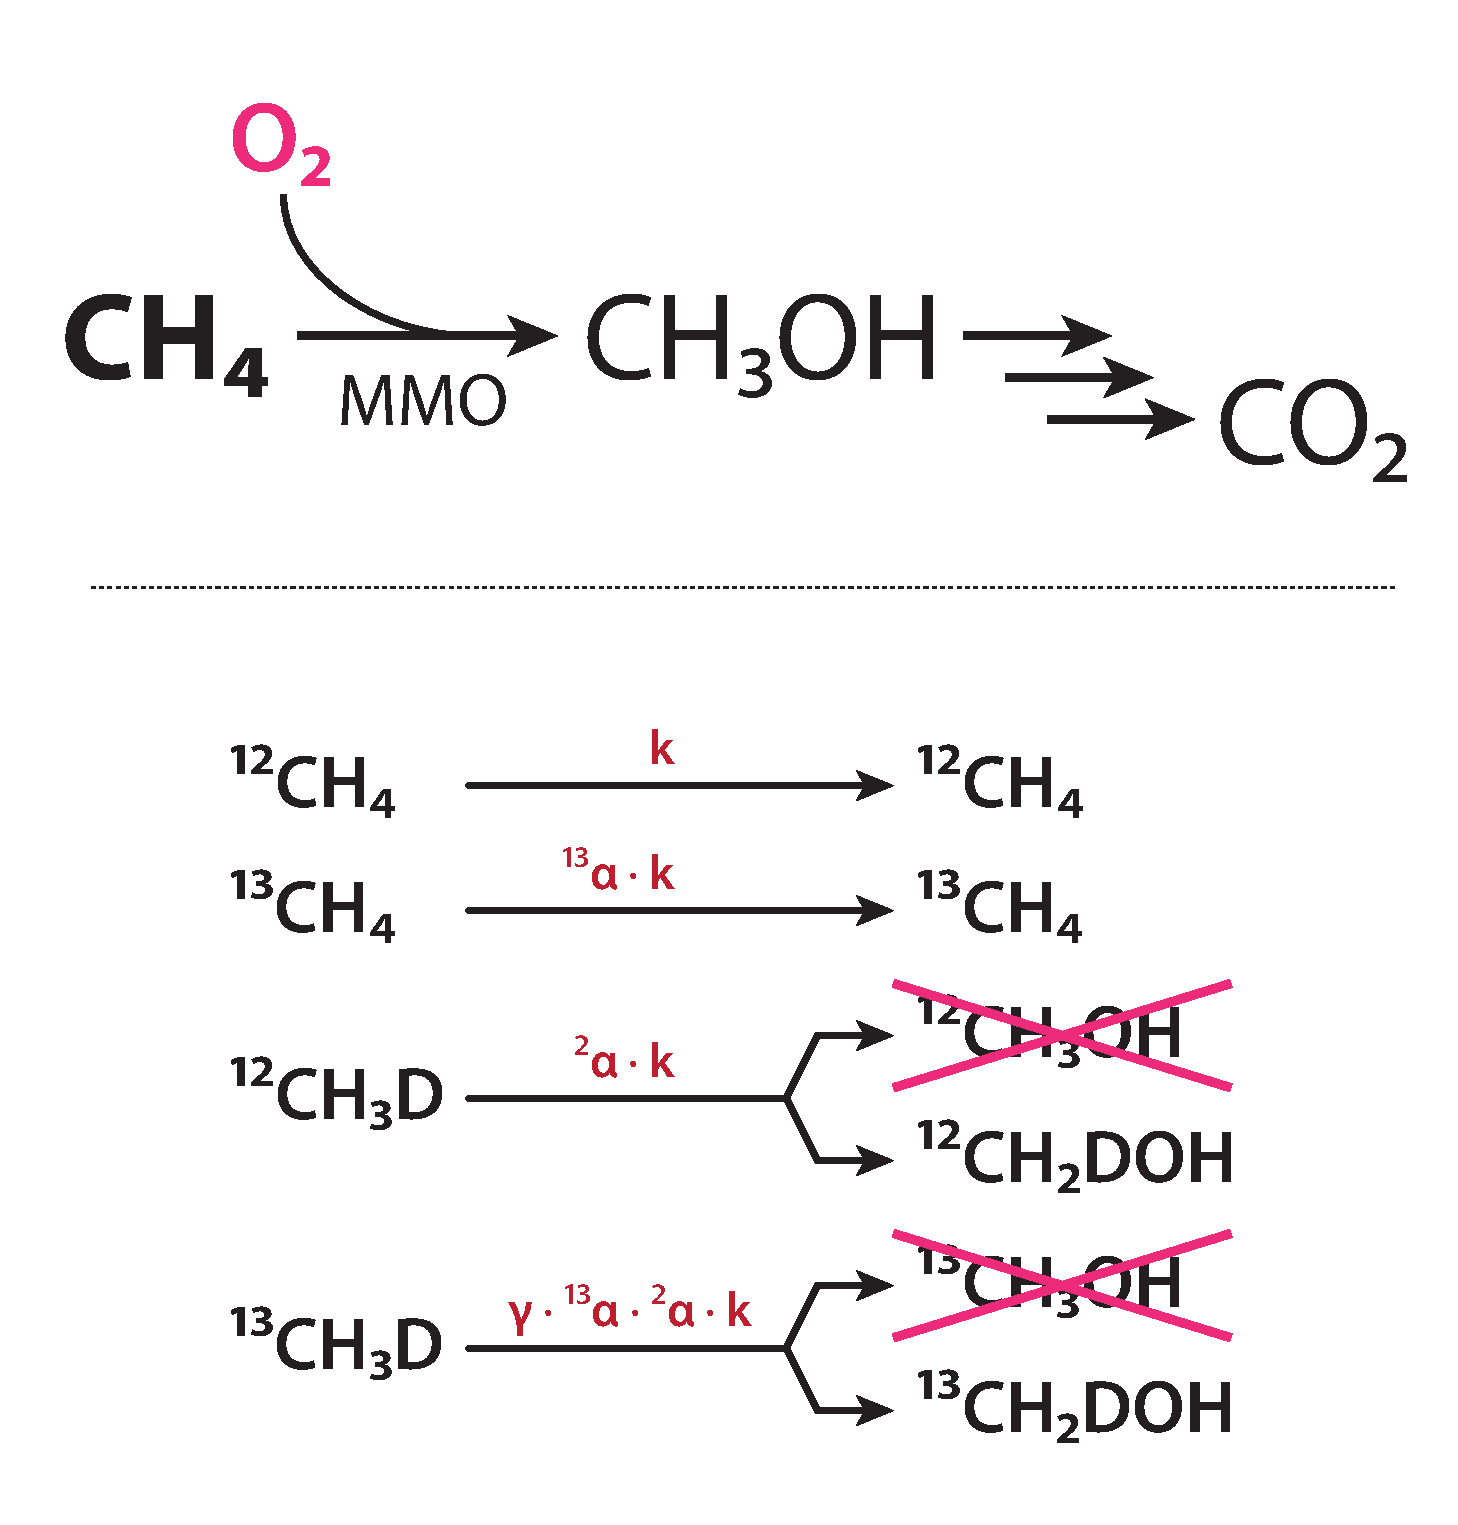
\includegraphics[width=0.45\textwidth]{figures/Fig1.8.pdf}
	\captionsetup{format=myformat}	% hrule beneath caption
	\caption[Reaction scheme for four stable isotopologues of methane during methane oxidation]{Reaction scheme for four stable isotopologues of
		methane during methane oxidation. Abstraction of D is
		\textasciitilde{}100× slower than H-abstraction. Substitution of D at an
		adjacent site has a small (\textasciitilde{}10\%)
		effect \parencite{Nesheim+Lipscomb_1996_Bc}. This means that
		the D/H fractionation comes mostly from the ¾ probability associated
		with abstraction of H from monodeuterated methane. 
		
		\quad \autoref{ch:4} and \textcite{Whitehill++_2017_GCA} show that
		fractionations are related by: 	\cee{\textsuperscript{13}CH\textsubscript{3}D/\textsuperscript{12}CH\textsubscript{4}
		= $\gamma$ × (\textsuperscript{13}C/\textsuperscript{12}C) × (D/H)},  where $\gamma$ is
		a number close to 1.000 (identical within error for OH and aerobic
		methanotrophy, and slightly less than 1 for Cl). Together, these
		fractionation factors constrain the effects on
		\textsuperscript{13}CH\textsubscript{3}D by the major methane sink
		reactions in the atmosphere and in oxic microbial habitats on Earth.}
	\label{fig:1:8}
\end{SCfigure*}
